% !TEX program = pdflatex
% Defensa TFM — Beamer (línea cronológica del documento)
\documentclass[aspectratio=169,10pt,professionalfonts]{beamer}

\usepackage[T1]{fontenc}
\usepackage[scaled=0.95]{helvet}
\renewcommand{\familydefault}{\sfdefault}
\usepackage{lmodern}
\renewcommand{\familydefault}{\sfdefault}
\usepackage[spanish]{babel}
\usepackage{amsmath,amssymb,bm}
\usepackage{booktabs}
\usepackage{tabularx}
\usepackage{graphicx}
\usepackage{tikz}
\usetikzlibrary{positioning,fit,arrows.meta,babel,calc}
\usepackage[authoryear,round]{natbib}

\graphicspath{{../Imagenes/}{../../POCs/data/output/figures/}{../}}

% ── Diseño alineado con la plantilla de defensa de UNIR (PowerPoint) ──
% Paleta de la plantilla: azul UNIR, azul oscuro, grises (sin verdes ni rojos).
\definecolor{unirazul}{HTML}{219BC3}
\definecolor{unirnavy}{HTML}{0E4A75}
\definecolor{unirgris}{HTML}{858591}
\definecolor{unirclaro}{HTML}{C0C0C8}
\definecolor{ink}{HTML}{3D3D4A}
% Los diagramas TikZ usan solo la paleta de la plantilla
\colorlet{blue}{unirazul}
\colorlet{orange}{unirnavy}
\colorlet{violet}{unirgris}

\usetheme{default}
\usefonttheme{professionalfonts}
\setbeamercolor{normal text}{fg=ink,bg=white}
\setbeamercolor{structure}{fg=unirazul}
\setbeamercolor{alerted text}{fg=unirnavy}
\setbeamercolor{block title}{bg=unirazul,fg=white}
\setbeamercolor{block body}{bg=unirazul!8}
\setbeamercolor{block title alerted}{bg=unirnavy,fg=white}
\setbeamercolor{block body alerted}{bg=unirnavy!8}
\setbeamerfont{block title}{series=\bfseries,size=\small}
\setbeamersize{text margin left=0.85cm,text margin right=0.85cm}
\setbeamertemplate{navigation symbols}{}
\setbeamertemplate{itemize item}{\textcolor{unirazul}{\small$\bullet$}}
\setbeamertemplate{itemize subitem}{\textcolor{unirazul}{\scriptsize$\circ$}}
\setbeamertemplate{enumerate items}[default]
\setbeamercolor{enumerate item}{fg=unirazul}
\addtobeamertemplate{itemize body begin}{}{\setlength{\itemsep}{1pt}\setlength{\parsep}{0pt}}
\addtobeamertemplate{enumerate body begin}{}{\setlength{\itemsep}{1pt}\setlength{\parsep}{0pt}}

% Título de diapositiva: línea azul (apartado) + línea verde azulada (título)
\makeatletter
\setbeamertemplate{frametitle}{%
  \vskip 0.30cm
  \edef\unir@sec{\detokenize\expandafter{\insertsectionhead}}%
  \edef\unir@ttl{\detokenize\expandafter{\insertframetitle}}%
  \ifx\unir@sec\unir@ttl
    {\fontsize{14}{16}\selectfont\bfseries\color{unirnavy}\insertframetitle\par}%
  \else
    {\fontsize{14}{16}\selectfont\bfseries\color{unirazul}\insertsectionhead\par}%
    {\fontsize{14}{16}\selectfont\bfseries\color{unirnavy}\insertframetitle\par}%
  \fi
  \vskip 0.12cm}
\makeatother
\setbeamerfont{frametitle}{size=\normalsize}

% Pie: logotipo UNIR a la izquierda y «pág. NN» con barra vertical a la derecha
\newcommand{\unirpagina}{%
  \begin{tikzpicture}[baseline=0pt]
    \draw[unirazul, line width=1.6pt] (0,-0.12) -- (0,0.50);
    \node[anchor=south west, font=\fontsize{8}{9}\selectfont\bfseries, text=unirclaro, align=left,
          inner sep=0pt] at (0.14,-0.12)
      {p\'ag.\\ \ifnum\insertframenumber<10 0\fi\insertframenumber};
  \end{tikzpicture}}
\setbeamertemplate{footline}{%
  \leavevmode\hbox to\paperwidth{%
    \hskip0.75cm\raisebox{0.10cm}{
\includegraphics[height=0.62cm]{logo_unir.png}}%
    \hfill\raisebox{0.14cm}{\unirpagina}\hskip0.85cm}%
  \vskip0.12cm}

\title{Ventaja cuántica en ciencia de datos:\\
condiciones empíricas, métodos híbridos\\
y criterios de activación selectiva}
\subtitle{Defensa del Trabajo de Fin de Máster}
\author{Juan David Prada Malagón}
\institute{Máster en Computación Cuántica · UNIR\\[2pt]
Director: Ricardo Rafael Domínguez Reyes}
\date{}

\begin{document}

% =====================================================================
\section{Título}
% =====================================================================
\begin{frame}[plain]
\begin{tikzpicture}[remember picture,overlay]
  \fill[unirazul] (current page.north west) rectangle ($(current page.south east)+(0,1.15)$);
  \node[text=white, align=center, text width=11cm, inner sep=0pt] (tt) at ($(current page.center)+(0,0.55)$)
    {{\fontsize{20}{24}\selectfont\bfseries\hyphenpenalty=10000 Ventaja cuántica en ciencia de datos:\\
      condiciones empíricas,\\ métodos híbridos y criterios\\ de activación selectiva\par}
     \vspace{0.55cm}
     {\large Defensa del Trabajo de Fin de Máster\par}
     \vspace{0.3cm}
     {\normalsize Juan David Prada Malagón\par}
     \vspace{0.12cm}
     {\footnotesize Máster en Computación Cuántica $\cdot$ UNIR\\ Director: Ricardo Rafael Domínguez Reyes\par}};
  \draw[white, line width=1.1pt] ($(tt.north west)+(-0.55,0.45)$) -- ++(0,-0.7) ($(tt.north west)+(-0.55,0.45)$) -- ++(0.7,0);
  \draw[white, line width=1.1pt] ($(tt.south east)+(0.55,-0.45)$) -- ++(0,0.7) ($(tt.south east)+(0.55,-0.45)$) -- ++(-0.7,0);
  \node[anchor=south west, inner sep=0pt] at ($(current page.south west)+(0.75,0.12)$)
    {
\includegraphics[height=0.82cm]{logo_unir.png}};
\end{tikzpicture}
\end{frame}

\begin{frame}[plain]
\begin{tikzpicture}[remember picture,overlay]
  \fill[unirazul] (current page.north west) rectangle (current page.south |- current page.south west);
  \fill[unirazul] (current page.north west) rectangle ($(current page.south)$);
  \node[text=white, anchor=west] at ($(current page.west)+(1.6,0)$) {{\fontsize{34}{38}\selectfont ÍNDICE}};
  \node[anchor=west, align=left, inner sep=0pt, font=\fontsize{11.5}{14}\bfseries\selectfont] at ($(current page.center)+(0.35,0)$)
    {
    \textcolor{unirclaro}{01 --}\,\textcolor{unirnavy}{Motivación}\\[0.30cm]
    \textcolor{unirclaro}{02 --}\,\textcolor{unirnavy}{Introducción}\\[0.30cm]
    \textcolor{unirclaro}{03 --}\,\textcolor{unirnavy}{Contexto y estado de la técnica}\\[0.30cm]
    \textcolor{unirclaro}{04 --}\,\textcolor{unirnavy}{Planteamiento y metodología}\\[0.30cm]
    \textcolor{unirclaro}{05 --}\,\textcolor{unirnavy}{Resultados: Q vs C}\\[0.30cm]
    \textcolor{unirclaro}{06 --}\,\textcolor{unirnavy}{Conjeturas: $\mathcal{Q}$ y QCR}\\[0.30cm]
    \textcolor{unirclaro}{07 --}\,\textcolor{unirnavy}{Evidencia de las conjeturas}\\[0.30cm]
    \textcolor{unirclaro}{08 --}\,\textcolor{unirnavy}{Conclusiones y limitaciones}\\[0.30cm]
    \textcolor{unirclaro}{09 --}\,\textcolor{unirnavy}{Trabajo futuro}
    };
\end{tikzpicture}
\end{frame}

% =====================================================================
\section{Motivación}
% =====================================================================
\begin{frame}{La brecha entre promesa y evidencia}
\begin{columns}[T]
\begin{column}{0.55\textwidth}
\begin{itemize}
  \item La ciencia de datos escala en dimensionalidad y complejidad combinatoria \citep{jordan2015, biamonte2017}.
  \item Los algoritmos variacionales y de kernel prometen ventaja en la era NISQ \citep{preskill2018, farhi2014, schuld2021}.
  \item Persiste una \textbf{brecha} entre promesas teóricas y evidencia reproducible sobre datos reales.
\end{itemize}
\end{column}
\begin{column}{0.42\textwidth}
\begin{block}{Pregunta práctica}
\textquestiondown{}Cuándo activar un módulo cuántico\\
y cuándo quedarse con el stack clásico?
\end{block}
\end{column}
\end{columns}
\end{frame}

\begin{frame}{Estructura del TFM}
\centering
\begin{tikzpicture}[font=\scriptsize, thick, scale=0.85, every node/.style={transform shape},
    capnodo/.style={rectangle, rounded corners=4pt, very thick,
                minimum width=2.8cm, minimum height=0.75cm,
                align=center, inner sep=3pt},
    bloque/.style={rectangle, rounded corners=6pt, dashed,
                   inner sep=6pt, very thick},
    arr/.style={->, thick, gray!60}]
  \node[capnodo, draw=blue!55!black, fill=blue!8]  (c1) at (0,    0) {\textbf{Cap. 1}\\Introducción};
  \node[capnodo, draw=blue!55!black, fill=blue!8]  (c2) at (0,  -1.35) {\textbf{Cap. 2}\\Contexto};
  \node[capnodo, draw=blue!55!black, fill=blue!8]  (c3) at (0,  -2.7) {\textbf{Cap. 3}\\Objetivos};
  \node[capnodo, draw=orange!60!black, fill=orange!7] (c4) at (4.6, -1.35) {\textbf{Cap. 4}\\Metodología};
  \node[capnodo, draw=orange!60!black, fill=orange!7] (c5) at (4.6, -2.7) {\textbf{Cap. 5}\\Evaluación};
  \node[capnodo, draw=violet!60!black, fill=violet!7] (c6) at (9.2, -0.8) {\textbf{Cap. 6}\\QCR / $\mathcal{Q}$};
  \node[capnodo, draw=violet!60!black, fill=violet!7] (c7) at (9.2, -2.15) {\textbf{Cap. 7}\\Conclusiones};
  \node[capnodo, draw=violet!60!black, fill=violet!7] (c8) at (9.2, -3.5) {\textbf{Cap. 8}\\Futuro};
  \node[bloque, draw=blue!40,   fit=(c1)(c2)(c3),
        label={[blue!60!black, font=\scriptsize\bfseries]above:Marco teórico}]   {};
  \node[bloque, draw=orange!45, fit=(c4)(c5),
        label={[orange!65!black, font=\scriptsize\bfseries]above:Implementación}] {};
  \node[bloque, draw=violet!45, fit=(c6)(c7)(c8),
        label={[violet!60!black, font=\scriptsize\bfseries]above:Discusión y cierre}] {};
  \draw[arr] (c3.east)  -- ++(0.55, 0) |- (c4.west);
  \draw[arr] (c4.south) -- (c5.north);
  \draw[arr] (c5.east)  -- ++(0.55, 0) |- (c6.west);
  \draw[arr] (c6.south) -- (c7.north);
  \draw[arr] (c7.south) -- (c8.north);
  \draw[->, thick, dashed, gray!50]
    (c5.north east) to[out=25, in=200] node[midway, above, font=\tiny, gray!65]{valida} (c6.south west);
\end{tikzpicture}
\end{frame}

% =====================================================================
\section{Introducción}
% =====================================================================
\begin{frame}{Planteamiento del problema}
El problema central del trabajo \citep{preskill2018, biamonte2017}:

\begin{quote}
\itshape
\textquestiondown{}En qué condiciones, y para qué tipos de problemas de ciencia de datos,
los algoritmos cuánticos disponibles en la era NISQ ofrecen una
ventaja real y medible frente a los algoritmos clásicos?
\end{quote}

\vspace{0.6em}
\begin{block}{Hipótesis operativa}
La ventaja es \textbf{real pero condicionada}:
\begin{enumerate}
  \item coincidencia \textbf{feature map} $\leftrightarrow$ \textbf{generador de datos}, o
  \item problema formulable como QUBO con arquitectura \textbf{híbrida} a escala viable.
\end{enumerate}
\end{block}
\end{frame}

\begin{frame}{Alcance}
\begin{columns}[T]
\begin{column}{0.5\textwidth}
\textbf{Familias industriales (4)}
\begin{itemize}
  \item Clasificación supervisada (QSVM)
  \item Regresión (QK-SVR)
  \item Optimización combinatoria (QAOA)
  \item Optimización / híbrido (VQE + MDS)
\end{itemize}
{\footnotesize Extendidas a 9 protocolos justos en el documento (anomalías, TSP, lags,\ldots).}
\end{column}
\begin{column}{0.48\textwidth}
\textbf{Tres capas de datos}
\begin{enumerate}
  \item Sintéticos con estructura cuántica nativa \citep{liu2021}
  \item Práctica SKG Tecnología
  \item Referencia pública
\end{enumerate}
\end{column}
\end{columns}
\end{frame}

% =====================================================================
\section{Contexto y estado de la técnica}
% =====================================================================
\begin{frame}{Era NISQ}
\begin{block}{NISQ \citep{preskill2018}}
Dispositivos de escala intermedia \textbf{ruidosos}: qubits limitados, decoherencia, sin corrección de errores a gran escala.
\end{block}
\begin{itemize}
  \item Algoritmos viables hoy: \textbf{variacionales} (QAOA, VQE) e híbridos \citep{farhi2014, cerezo2021}.
  \item Kernels cuánticos: acceso a espacios de Hilbert de alta dimensión \citep{schuld2021, huang2021}.
  \item Distinción clave: \textbf{metodologías} maduras vs.\ \textbf{hardware} aún inmaduro.
\end{itemize}
\end{frame}

\begin{frame}{Comparaciones cuántico--clásico en la literatura}
\begin{itemize}
  \item Condiciones teóricas de ventaja de kernel: geometría de datos crítica \citep{huang2021}.
  \item Datasets donde el kernel cuántico es óptimo por construcción \citep{liu2021}.
  \item Concentración de kernels y límites prácticos \citep{thanasilp2022}.
  \item Gap empírico: pocos estudios \textbf{justos} sobre datos empresariales reales \citep{fastovets2019}.
\end{itemize}
\begin{alertblock}{Posicionamiento de este TFM}
Evidencia empírica + protocolos justos + diagnóstico $\mathcal{Q}(\mathcal{D})$ + QCR formalmente planteado.
\end{alertblock}
\end{frame}

% =====================================================================
\section{Planteamiento y metodología}
% =====================================================================
\begin{frame}{Metodología en cuatro fases}
\centering
\begin{tikzpicture}[font=\footnotesize,
    fase/.style={rectangle, rounded corners=4pt, very thick,
                 minimum width=11.2cm, minimum height=0.95cm,
                 align=center, inner sep=5pt},
    arr/.style={->, very thick, >=stealth}]
  \node[fase, draw=blue!60!black, fill=blue!9] (f1) {
    \textbf{Fase 1 --- Datos:} nativo / SKG / público $\cdot$ normalización $\cdot$ PCA};
  \node[fase, draw=orange!60!black, fill=orange!9, below=0.35cm of f1] (f2) {
    \textbf{Fase 2 --- Algoritmos:} QSVM $\cdot$ QK-SVR $\cdot$ QAOA $\cdot$ VQE vs.\ GB / RF / RBF};
  \node[fase, draw=unirnavy!70!black, fill=unirnavy!9, below=0.35cm of f2] (f3) {
    \textbf{Fase 3 --- Evaluación:} CV $\cdot$ Acc / F1 / $R^2$ / AUC $\cdot$ escalabilidad};
  \node[fase, draw=violet!60!black, fill=violet!9, below=0.35cm of f3] (f4) {
    \textbf{Fase 4 --- Híbrido:} integración QAOA--COBYLA $\cdot$ criterios de activación $\cdot$ QCR};
  \draw[arr] (f1)--(f2); \draw[arr] (f2)--(f3); \draw[arr] (f3)--(f4);
\end{tikzpicture}
\end{frame}

\begin{frame}{Diseño: 4 familias $\times$ 3 capas de datos}
\centering
\renewcommand{\arraystretch}{1.1}
\begin{tabular}{@{}lll@{}}
\toprule
\textbf{Familia} & \textbf{Cuántico} & \textbf{Clásico de referencia} \\
\midrule
Clasificación & QSVM (ZZ) & GB, RF, SVM-RBF \\
Regresión & QK-SVR & RF, XGBoost, SVR-RBF, Ridge \\
Anomalías & OCSVM-ZZ & IsolationForest, LOF \\
Optimización & QAOA / VQE & Greedy, ILP, NN+2-opt \\
\bottomrule
\end{tabular}

\vspace{0.4em}
Misma pregunta en las cuatro: \textbf{\textquestiondown{}quién gana, Q o C?}
en (i)~\textbf{cuántico-nativo}, (ii)~\textbf{SKG}, (iii)~\textbf{referencia}.

\vspace{0.2em}
\begin{block}{Lectura transversal}
Kernels: ventaja si mapa y generador coinciden.
Optimización: QUBO + híbrido a escala viable (no speedup asintótico).
\end{block}
\end{frame}

\begin{frame}{Criterio de activación del módulo cuántico}
\centering
{\footnotesize
\renewcommand{\arraystretch}{1.15}
\begin{tabular}{@{}p{2.6cm}p{3.6cm}p{3.2cm}p{3.0cm}@{}}
\toprule
\textbf{Problema} & \textbf{Activar si} & \textbf{Módulo Q} & \textbf{Fallback} \\
\midrule
Clasif.\ /\ Regresión &
coincidencia mapa--generador
\emph{y} vence a GB/RF
(no basta $\mathcal{Q}>0$ vs RBF) &
QSVM / QK-SVR &
GB / RF \\
Anomalías &
novedad alineada al mapa
(\texttt{zz\_phase}) &
OCSVM-ZZ &
IF / LOF \\
Forecasting &
target alineado (\texttt{zz\_lag}) &
QK-SVR &
Ridge / GB \\
Optimización / TSP &
QUBO factible, $n$ viable &
QAOA / VQE &
Greedy / ILP / 2-opt \\
Caso general &
SKG/Telco sin estructura ZZ
o $n$ demasiado grande &
\textbf{no se activa} &
pipeline clásico \\
\bottomrule
\end{tabular}}
\end{frame}

% =====================================================================
\section{Resultados: Q vs C}
% =====================================================================
\begin{frame}{Qué comparamos}
\centering
{\small
\renewcommand{\arraystretch}{1.3}
\begin{tabular}{@{}lccc@{}}
\toprule
\textbf{Familia} & \textbf{Nativo} & \textbf{SKG} & \textbf{Referencia} \\
\midrule
1. Clasificación (QSVM) & Liu ZZ & Incidentes Bogotá & Telco Churn \\
2. Regresión (QK-SVR) & target alineado & Movilidad Bogotá & Friedman \#1 \\
3. Anomalías (OCSVM-ZZ) & \texttt{zz\_phase} & outliers inyectados & moons \\
4. Optimización (QAOA) & asignación QUBO & cobertura MDS & TSP $n{=}4$ \\
\bottomrule
\end{tabular}}
\vspace{1em}
\begin{block}{Formato fijo en las 4 diapositivas siguientes}
Plot (o tabla) + misma lectura: \textbf{Nativo / SKG / Referencia} $\rightarrow$ gana Q o gana C.
Sin formalismo, sin ejemplos narrativos, sin algoritmos fuera del TFM.
\end{block}
\end{frame}

% --- 1. Clasificación ------------------------------------------------
\begin{frame}{1. Clasificación (QSVM vs clásico)}
\begin{columns}[T]
\begin{column}{0.68\textwidth}
\centering
\includegraphics[width=\linewidth,height=0.72\textheight,keepaspectratio]{06_quantum_kernel_3datasets_comparativa.png}
\end{column}
\begin{column}{0.30\textwidth}
\begin{block}{Q vs C}
\begin{itemize}
  \item \textbf{Nativo:} gana Q\\{\footnotesize(+13.3\,pp)}
  \item \textbf{SKG:} gana C\\{\footnotesize($-6.0$\,pp)}
  \item \textbf{Telco:} gana C\\{\footnotesize($-3.8$\,pp vs GB)}
\end{itemize}
\end{block}
{\footnotesize Baseline = mejor clásico.
También: Q más lento ($1/t\approx 0$).}
\end{column}
\end{columns}
\end{frame}

% --- 2. Regresión ----------------------------------------------------
\begin{frame}{2. Regresión (QK-SVR vs clásico)}
\begin{columns}[T]
\begin{column}{0.68\textwidth}
\centering
\includegraphics[width=\linewidth,height=0.72\textheight,keepaspectratio]{03_regresion_3datasets.png}
\end{column}
\begin{column}{0.30\textwidth}
\begin{block}{Q vs C}
\begin{itemize}
  \item \textbf{Nativo:} gana Q\\{\footnotesize($\Delta R^2{=}{+}0.60$)}
  \item \textbf{Friedman:} gana C\\{\footnotesize($\Delta R^2{=}{-}0.13$)}
  \item \textbf{SKG:} gana C\\{\footnotesize($\Delta R^2{=}{-}0.34$)}
\end{itemize}
\end{block}
{\footnotesize Misma lectura que clasificación:
ventaja solo con estructura alineada.}
\end{column}
\end{columns}
\end{frame}

% --- 3. Anomalías ----------------------------------------------------
\begin{frame}{3. Anomalías (OCSVM-ZZ vs clásico)}
\begin{columns}[T]
\begin{column}{0.68\textwidth}
\centering
\includegraphics[width=\linewidth,height=0.72\textheight,keepaspectratio]{08_anomaly_3datasets_comparativa.png}
\end{column}
\begin{column}{0.30\textwidth}
\begin{block}{Q vs C}
\begin{itemize}
  \item \textbf{Nativo:} gana Q\\{\footnotesize(+31.2\,pp AUC)}
  \item \textbf{SKG:} gana C\\{\footnotesize($-29.9$\,pp)}
  \item \textbf{moons:} gana C\\{\footnotesize($-29.1$\,pp)}
\end{itemize}
\end{block}
{\footnotesize Misma lectura que clasif./regresión:
ventaja solo con novedad alineada al mapa.}
\end{column}
\end{columns}
\end{frame}

% --- 4. Optimización -------------------------------------------------
\begin{frame}{4. Optimización (QAOA/VQE vs clásico)}
\centering
{\small
\renewcommand{\arraystretch}{1.1}
\begin{tabular}{@{}lccc@{}}
\toprule
\textbf{Capa} & \textbf{Problema} & \textbf{Cuántico} & \textbf{Clásico} \\
\midrule
Nativo / control &
Asignación QUBO &
\textbf{QAOA $-$30.3\% coste} &
Greedy \\
SKG-like &
MDS (cobertura) &
\textbf{óptimo; $P\!\approx\!73\%$} &
fuerza bruta / Greedy \\
Referencia &
TSP $n{=}4$ &
empate óptimo &
NN+2-opt (gap $0$) \\
\bottomrule
\end{tabular}}
\vspace{0.4em}
\begin{block}{Q vs C (misma pregunta)}
\begin{itemize}
  \item \textbf{Asignación:} gana Q en coste a escala moderada.
  \item \textbf{MDS:} Q recupera el óptimo (patrón híbrido viable).
  \item \textbf{TSP:} empate en calidad; \textbf{no} hay speedup --- modelado QUBO.
\end{itemize}
\end{block}
{\footnotesize Optimización $\neq$ kernels: aquí el contraste es coste/calidad de solución, no accuracy.
La estructura del paisaje QUBO se mide aparte (P1, notebook~11).}
\end{frame}

% --- Síntesis compacta -----------------------------------------------
\begin{frame}{Síntesis 4 $\times$ 3}
\centering
{\small
\renewcommand{\arraystretch}{1.25}
\begin{tabular}{@{}lccc@{}}
\toprule
\textbf{Familia} & \textbf{Nativo} & \textbf{SKG} & \textbf{Referencia} \\
\midrule
Clasificación & \textbf{gana Q} & gana C & gana C \\
Regresión & \textbf{gana Q} & gana C & gana C \\
Anomalías & \textbf{gana Q} & gana C & gana C \\
Optimización & \textbf{gana Q} (coste) & \textbf{viable} (óptimo) & empate \\
\bottomrule
\end{tabular}}
\vspace{0.8em}
\begin{block}{Mensaje único}
Ventaja cuántica \textbf{condicionada}: aparece con alineación mapa--generador
(o QUBO viable). En datos reales SKG/Telco sin esa estructura: pipeline clásico.
\end{block}
\end{frame}

% =====================================================================
\section{Conjeturas}
% =====================================================================
\begin{frame}{De la evidencia emergen dos preguntas}
\begin{block}{Preguntas originales (Cap.~6)}
\begin{enumerate}
  \item \textbf{P1 --- tests de cuanticidad}\\[0.35em]
        \textquestiondown{}Se puede diagnosticar \emph{a priori} si un dataset tiene
        \emph{estructura cuántica} (alineación mapa--dato) y, por tanto, admitirá ventaja?

  \vspace{1.0em}
  \item \textbf{P2 --- mapeos cuántico-compatibles}\\[0.35em]
        Si no hay estructura nativa, \textquestiondown{}existe un nuevo mapeo $\psi$ y un espacio
        de representación donde se conserve la estructura e información del dato,
        adquiera estructura cuántica, y haya mapa de vuelta si hace falta?
        (analogía: Fourier)
\end{enumerate}
\end{block}
\end{frame}

\begin{frame}{Camino a la Conjetura 1 (I) --- por qué un perfil}
\begin{columns}[T]
\begin{column}{0.48\textwidth}
\begin{block}{Literatura}
\begin{itemize}
  \item Ventaja cuántica de kernel $\Rightarrow$
        alineación con etiquetas \textbf{y}
        geometría no reproducible por el
        clásico \citep{huang2021, liu2021}.
  \item Un solo indicador no basta:
        hace falta $A_Q > A_{cl}$
        \textbf{y} $d_F$ grande
        \citep{huang2021, schuld2021}.
  \item Riesgo: el kernel cuántico puede
        \textbf{concentrarse} y perder señal
        --- vigilar $H(K)$ \citep{thanasilp2022}.
\end{itemize}
\end{block}
\end{column}
\begin{column}{0.48\textwidth}
\begin{block}{Hecho empírico}
Ventaja si el mapa que estructura el dato
= mapa del modelo \textbf{cuántico}.
Si no: gana el \textbf{clásico}.
\end{block}
\vspace{0.5em}
\begin{block}{Idea corregida}
No un escalar: un \textbf{vector}
$\mathcal{Q}(\mathcal{D})=(\Delta A,\hat{d}_F,\Delta H,\hat g,\ldots)$
que se \emph{mira} componente a componente.
\end{block}
\end{column}
\end{columns}
\end{frame}

\begin{frame}{Camino a la Conjetura 1 (II) --- componentes y evidencia}
\begin{columns}[T]
\begin{column}{0.58\textwidth}
\begin{block}{Interpretación (cuántico vs clásico)}
{\footnotesize
\begin{itemize}
  \item $\Delta A$ --- \textquestiondown{}el cuántico ve mejor las clases?\\
        $>0$: sí, más alineación con las etiquetas
        que el clásico \citep{cortes2012, huang2021}.
  \item $\hat{d}_F$ --- \textquestiondown{}la geometría es distinta?\\
        Grande: el cuántico no es un clásico
        disfrazado \citep{liu2021}.
  \item $\Delta H$ --- \textquestiondown{}el kernel cuántico aporta
        diversidad o se ha ``aplanado''?\\
        Bajo/negativo: todas las similitudes se parecen
        (concentración) $\Rightarrow$ poca info útil
        \citep{thanasilp2022}.
  \item $\hat g$ --- \textquestiondown{}el RBF reproduce la geometr\'ia
        cu\'antica?\\
        Cerca de $1$: s\'i; grande: no (necesario, no suficiente)
        \citep{huang2021}.
\end{itemize}}
\end{block}
\end{column}
\begin{column}{0.40\textwidth}
\begin{block}{Evidencia (TFM)}
Barrido $\alpha$ ($n{=}9$, NB08):
mezcla de etiquetas, $X$ fijo.\\[0.25em]
Hallazgo robusto:
$\rho_S(\alpha,\Delta A){=}0.833$
($p{=}0.005$).\\[0.25em]
{\footnotesize $d_F$/$H$ constantes por diseño;
no confundir con
$\rho(\mathcal{Q},\mathrm{ventaja})$.}
\end{block}
\end{column}
\end{columns}
\end{frame}

\begin{frame}{Conjetura 1 --- $\mathcal{Q}(\mathcal{D})$ como \textbf{vector}, no escalar}
\begin{equation}
  \mathcal{Q}(\mathcal{D})
  \;=\;
  \bigl(\Delta A,\; \hat{d}_F,\; \Delta H,\; \hat g\bigr)
  \qquad\text{(perfil; sin pesos)}
  \label{eq:Q}
\end{equation}
{\footnotesize
Opcional en el documento: un escalar $w^\top\mathcal{Q}$ se probó y \textbf{falla} como ranking
operativo --- por eso no se usa para decidir.}

\vspace{0.4em}
\begin{columns}[T]
\begin{column}{0.48\textwidth}
\begin{block}{Cómo se lee}
{\footnotesize
\begin{itemize}
  \item $\Delta A$: \textquestiondown{}mejor alineación
        que el clásico?
  \item $\hat{d}_F$: \textquestiondown{}geometría distinta?
  \item $\Delta H$: \textquestiondown{}diversidad o
        concentración?
  \item $\hat g$: \textquestiondown{}el RBF reproduce
        la geometr\'ia cu\'antica?
\end{itemize}}
\end{block}
\end{column}
\begin{column}{0.48\textwidth}
\begin{alertblock}{Límite}
{\footnotesize
El vector describe geometría vs.\ RBF.
La adopción exige ventaja vs.\
mejor clásico \textbf{en la familia}
(clasif./reg./anomalías) y alineación
mapa--generador.}
\end{alertblock}
\end{column}
\end{columns}
\end{frame}

\begin{frame}{Validación P1 --- barrido sintético ($\alpha$)}
\begin{columns}[T]
\begin{column}{0.62\textwidth}
\centering
\includegraphics[width=\linewidth,height=0.68\textheight,keepaspectratio]{08_barrido_sintetico_alpha.png}
\end{column}
\begin{column}{0.36\textwidth}
\begin{block}{Qué es (NB08 real)}
{\footnotesize
\begin{itemize}
  \item $\alpha$: fracción de etiquetas
        cuánticas ($X$ fijo).
  \item $\Delta A$ crece con $\alpha$:
        $\rho_S{=}0.833$ ($p{=}0.005$).
  \item $d_F$ y $H$ \textbf{constantes}
        (kernels no cambian con labels).
\end{itemize}}
\end{block}
\begin{alertblock}{Límite}
{\footnotesize
$\rho{=}0.833$ es $\rho(\alpha,\Delta A)$,
no $\rho(\mathcal{Q},\text{ventaja})$.
Barrido structure-aware: trabajo futuro.}
\end{alertblock}
\end{column}
\end{columns}
\end{frame}

\begin{frame}{P1 --- qué comparamos (mismas métricas)}
\begin{block}{Estructura cuántica = vector $(\Delta A,\ \Delta H,\ d_F,\ g,\ \mathcal{Q})$}
{\footnotesize
\begin{itemize}
  \item $\Delta A = A(K_Q,yy^\top)-A(K_{\mathrm{RBF}},yy^\top)$ --- \citep{huang2021}
  \item $\Delta H = H(K_Q)-H(K_{\mathrm{RBF}})$ --- \citep{thanasilp2022}
  \item $d_F=\|K_Q-K_{\mathrm{RBF}}\|_F/n$ --- \citep{liu2021}
  \item $g$ (diferencia geom.) --- \citep{huang2021}; $\mathcal{Q}$ compuesto (este TFM)
\end{itemize}
\textbf{Mismo protocolo} en clasificación, regresión, anomalías y optimización
(ZZ 2q, $n{=}60$, 3 repeats, RBF Frobenius-best).\\
Optimización = \textbf{paisaje QUBO} (bitstrings $\to$ energía), no QAOA.\\
Control nulo: $\Delta A$ con $y$ permutada. Sin accuracy / $R^2$ / AUC / coste.}
\end{block}
\vspace{0.2em}
\begin{alertblock}{Nota: no hay $\Delta_{\mathrm{op}}$ aquí}
{\footnotesize
Eso era solo un nombre confuso para
``accuracy(QSVM)$-$accuracy(mejor clásico)'' en clasificación.
\textbf{No} es métrica de estructura. Se retiró de estas figuras.}
\end{alertblock}
\end{frame}

\begin{frame}{P1 --- qué mide $g$ (Huang et al., 2021)}
\begin{columns}[T]
\begin{column}{0.56\textwidth}
\centering
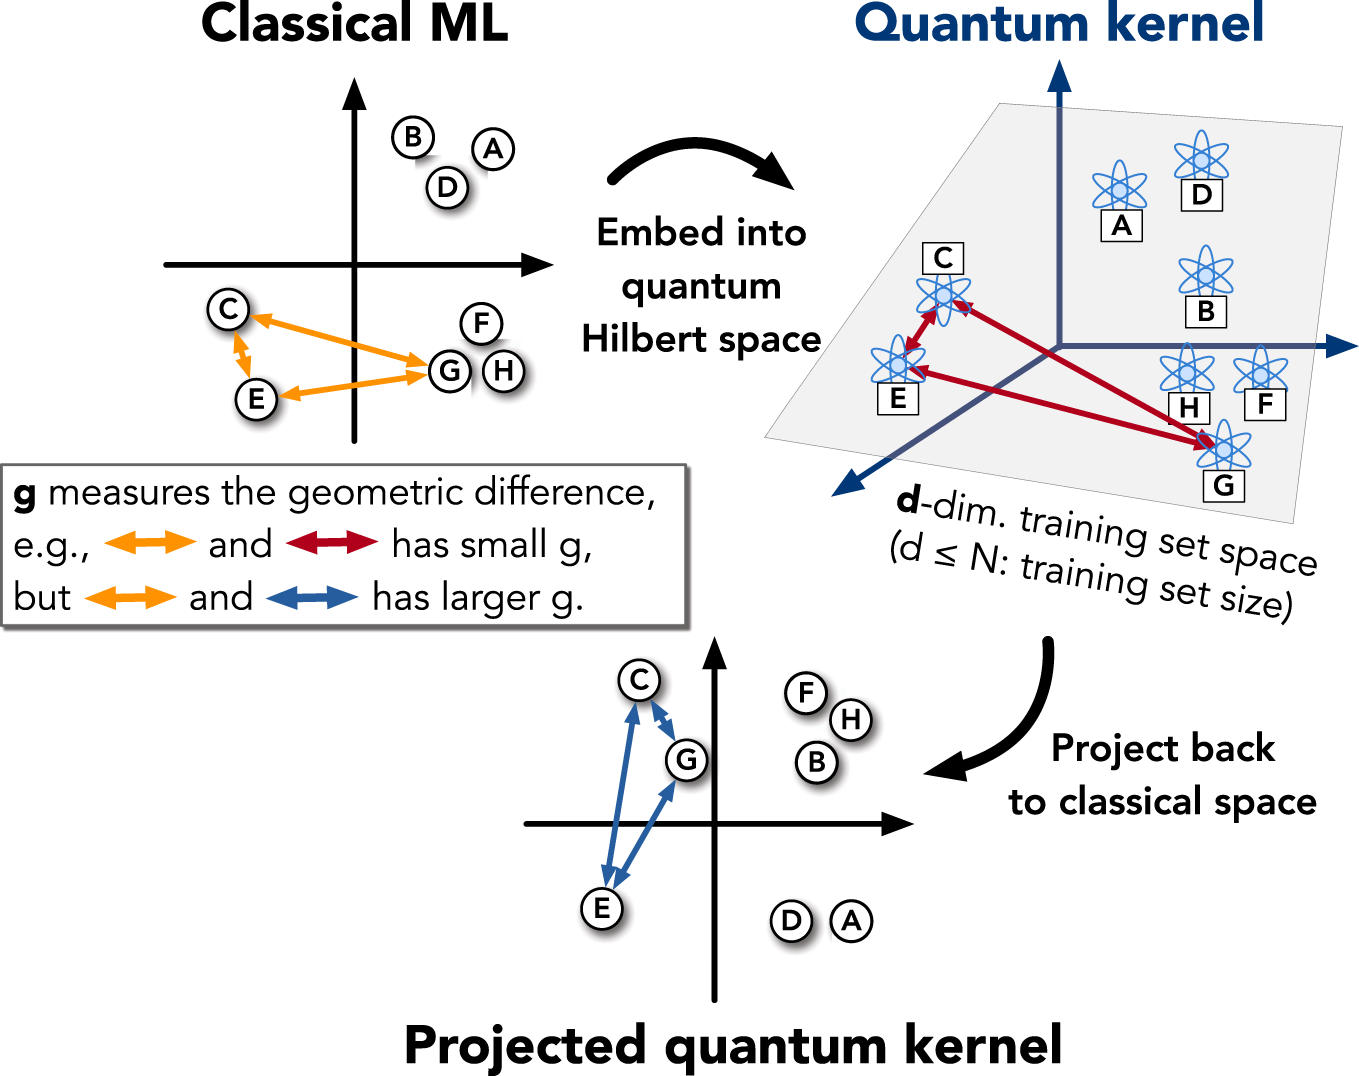
\includegraphics[width=\linewidth,height=0.56\textheight,keepaspectratio]{huang2021_fig2_geometria_kernel.png}\\[-0.2em]
{\tiny Fig.~2 de \citet{huang2021}, CC~BY~4.0}
\end{column}
\begin{column}{0.42\textwidth}
\begin{block}{Idea}
{\footnotesize
$g$ compara las \textbf{flechas} (similitudes kernel) entre puntos en el espacio
cl\'asico y en el cu\'antico. $g$ peque\~no: el kernel cl\'asico ya reproduce
la geometr\'ia cu\'antica; $g$ grande: no.\\[0.3em]
$d$ = dimensi\'on efectiva del dato en Hilbert.}
\end{block}
\begin{alertblock}{Nuestra medici\'on}
{\scriptsize
$g$: necesario, no suficiente; no usa $y$.
Huang ($\lambda{=}10^{-3}$): $g\approx 76$--$85$ en casi todos los casos
(42 en anomal\'ias-SKG, artefacto). $g\gg1$ pero igual para nativos y reales:
\textbf{no discrimina}. Antes $\approx 3000$ (artefacto).}
\end{alertblock}
\end{column}
\end{columns}
\end{frame}

\begin{frame}{P1 --- los cinco indicadores en los cuatro casos de uso}
\begin{columns}[T]
\begin{column}{0.66\textwidth}
\centering
\includegraphics[width=\linewidth,height=0.70\textheight,keepaspectratio]{08_estructura_comparativa_casos_uso.png}
\end{column}
\begin{column}{0.32\textwidth}
\begin{block}{Cómo leerlo}
{\footnotesize
Un panel por indicador; eje X = caso de uso;
3 barras = Nativo / SKG / Referencia
(optimizaci\'on: asignaci\'on / MaxCut / TSP).\\[0.3em]
\begin{itemize}
  \item $\Delta A$: solo los nativos superan el ruido (banda azul);
        el resto, dentro del ruido o por debajo (incluida la optimizaci\'on)
  \item $\Delta H$, $d_F$, $g$: casi planos;
        excepci\'on anomal\'ias-SKG = artefacto de escala (outliers $8\sigma$ comprimen el MinMax)
  \item $\mathcal{Q}$: informativo; lo dominan indicadores planos
\end{itemize}}
\end{block}
\end{column}
\end{columns}
\end{frame}

\begin{frame}{P1 --- cómo interpretar}
\begin{block}{\textquestiondown{}$\Delta A$ negativo + $\Delta H$ mínimo = estructura?}
{\footnotesize
\textbf{No.} Los \textbf{nativos} tienen $\Delta A>0$ sobre el ruido
(clasif.\ $+0.20$, reg.\ $+0.28$, anom.\ $+0.09$); los datos reales y los
paisajes de optimizaci\'on quedan dentro o por debajo del nulo
($\Delta A<0$ = el RBF alinea mejor, no ``estructura negativa'').
El \'unico $\Delta H$ m\'inimo (anomal\'ias-SKG, $0.44$) es un artefacto de escala.}
\end{block}
\vspace{0.35em}
\begin{block}{\textquestiondown{}$d_F$ discrimina?}
{\footnotesize
\textbf{Aqu\'i, apenas}: $\approx 0.01$ en todos los casos; $g$ y $\Delta H$ tambi\'en planos.
Solo $\Delta A$ usa $y$; los otros tres solo ven $X$.}
\end{block}
\vspace{0.35em}
\begin{alertblock}{Lectura defendible}
{\footnotesize
Lo que separa estructura es $\Delta A$ (alineaci\'on mapa--dato \citep{liu2021,huang2021}),
no $d_F$, $g$ ni $\Delta H$. Optimizaci\'on: paisaje QUBO con 2 qubits
(PCA retiene $\approx 1/3$): \textbf{sin evidencia} de estructura; l\'imite del dise\~no.}
\end{alertblock}
\end{frame}

\begin{frame}{Camino a la Conjetura 2 --- la analogía de Fourier}
\begin{columns}[T]
\begin{column}{0.52\textwidth}
\begin{block}{La pregunta natural de un matemático}
{\footnotesize
Un problema dif\'icil en el dominio original se vuelve simple en otro espacio,
y se regresa si hace falta. Ejemplo: la transformada de Fourier
$\hat f(\omega)=\int f(x)\,e^{-i\omega x}\,dx$
convierte convoluci\'on en producto.\\[0.3em]
Tres propiedades la hacen \'util: \textbf{conserva la informaci\'on} (invertible);
la \textbf{estructura se ve} (se vuelve diagonal); tiene \textbf{mapa de vuelta}.}
\end{block}
\end{column}
\begin{column}{0.44\textwidth}
\begin{block}{Y no es un mapa arbitrario}
{\footnotesize
Viene de un \textbf{n\'ucleo} (kernel) $e^{-i\omega x}$.
Por el teorema de Bochner, los kernels invariantes por traslaci\'on
son transformadas de Fourier de una medida:
el mapa de caracter\'isticas de un kernel \emph{es} un mapeo de tipo Fourier.}
\end{block}
\end{column}
\end{columns}
\vspace{0.1em}
\begin{alertblock}{La analog\'ia con el kernel cu\'antico}
{\footnotesize
Si el dato no tiene estructura cu\'antica, \textquestiondown{}existe un \textbf{nuevo mapeo $\psi$ y un espacio de
representaci\'on $\mathcal{Z}$} donde se conserve la estructura e informaci\'on del dato,
adquiera estructura cu\'antica y se pueda sacar partido de los algoritmos cu\'anticos,
con un mapeo de vuelta al espacio original cuando haga falta?}
\end{alertblock}
\end{frame}

\begin{frame}{Conjetura 2 --- espacio de representaci\'on QCR}
\begin{center}
\begin{tikzpicture}[font=\footnotesize, thick,
    box/.style={rectangle, rounded corners=3pt, draw=blue!55!black, fill=blue!8,
                minimum width=2.4cm, minimum height=0.7cm, align=center}]
  \node[box] (X) at (0,0) {Espacio original\\$\mathcal{X}$};
  \node[box, minimum width=3.6cm] (Z) at (5.2,0) {Representaci\'on cu\'antica\\$\mathcal{Z}$};
  \node[box] (Y) at (10.2,0) {Resultado\\$\hat y$ o soluci\'on};
  \draw[->, very thick] (X) -- node[above]{$\psi$} (Z);
  \draw[->, very thick] (Z) -- node[above]{$f_Q$} (Y);
  \draw[->, dashed, thick] (Y.south) to[bend left=10] node[below]{$\rho$ (si hace falta)} (X.south);
\end{tikzpicture}
\end{center}
\vspace{-1.3em}
\begin{columns}[T]
\begin{column}{0.50\textwidth}
\begin{block}{Qu\'e se pide de $\psi$}
{\footnotesize
\begin{enumerate}
  \item \textbf{Conserva estructura e informaci\'on} de los datos.
  \item \textbf{Estructura cu\'antica}: $\mathcal{Q}(\psi(\mathcal{D}))>0$.
  \item \textbf{Mapa de vuelta} $\rho$ al espacio original cuando se necesite
        (p.\,ej.\ optimizaci\'on).
  \item Utilidad: $\varepsilon(f_Q^\star\circ\psi)\le\varepsilon(f_C^\star)$.
\end{enumerate}
}
\end{block}
\end{column}
\begin{column}{0.47\textwidth}
\begin{block}{Sobre la naturaleza de $\psi$}
{\footnotesize
$\psi$ \textbf{no tiene por qu\'e ser un polinomio}: Fourier usa exponenciales
y nace de un kernel. Con ventaja global, el coste de calcular $\psi$ debe contarse.}
\end{block}
\begin{alertblock}{Estado}
{\footnotesize
Conjetura \textbf{abierta}: este TFM la \textbf{plantea}.
Prototipos (NB~09): sin ventaja frente al cl\'asico fuerte. Sin demostraci\'on.}
\end{alertblock}
\end{column}
\end{columns}
\end{frame}

% =====================================================================
\section{Conclusiones}
% =====================================================================
\begin{frame}{Conclusiones (I) --- ventaja condicionada}
\begin{enumerate}
  \item La ventaja cuántica en ciencia de datos es \textbf{real pero condicionada}.
  \item En kernels: aparece cuando el feature map coincide con el generador
        (ZZ medido aquí; Pauli-Y confirma el mismo principio).
  \item En \textbf{datos reales} SKG/Telco \textbf{sin} esa estructura: gana el \textbf{clásico}
        (no son cuántico-nativos).
  \item Regresión: ventaja acotada (Friedman); en movilidad SKG, el clásico domina.
  \item Anomalías / lags: misma regla --- solo con target alineado
        (\texttt{zz\_phase}, \texttt{zz\_lag}).
\end{enumerate}
\end{frame}

\begin{frame}{Conclusiones (II) --- híbridos y coste}
\begin{enumerate}
  \setcounter{enumi}{5}
  \item QAOA reduce coste de asignación $\approx 30\%$ vs.\ Greedy a escala moderada.
  \item VQE competitivo en portafolio pequeño; TSP $n{=}4$: empate óptimo
        (valor de \emph{modelado}, no speedup).
  \item MDS: patrón híbrido viable ($P(\mathrm{opt})\approx 73\%$).
  \item Coste de simulación del kernel $O(n^2)$: obstáculo práctico actual.
  \item Metodologías maduras vs.\ hardware inmaduro: resultados mixtos son esperables en NISQ.
\end{enumerate}
\end{frame}

\begin{frame}{Conclusiones (III) --- conjeturas y adopción}
\begin{enumerate}
  \setcounter{enumi}{10}
  \item $\mathcal{Q}(\mathcal{D})$ como \textbf{vector} $(\Delta A,\hat{d}_F,\Delta H,\hat g)$;
        el escalar colapsado no se usa; sí $\rho_S(\alpha,\Delta A){=}0.833$.
  \item QCR: \textbf{planteado}; evidencia preliminar vs.\ RBF; no rescate operativo.
  \item Adopción recomendada: \textbf{selectiva e híbrida} --- módulo cuántico como
        herramienta adicional, no sustituto del stack clásico (SKG).
\end{enumerate}
\vspace{0.6em}
\begin{block}{Respuesta a la pregunta del TFM}
Ventaja medible hoy cuando hay coincidencia mapa--generador o QUBO híbrido viable;
en ausencia de eso, el clásico domina --- y eso también es un resultado.
\end{block}
\end{frame}

\begin{frame}{Limitaciones (I)}
\begin{itemize}
  \item \textbf{Simulación statevector}: sin ruido NISQ de hardware; ideales $\neq$ shots reales.
  \item \textbf{PCA a $n_q{=}2$}: $\sim$68\% de varianza descartada; $\mathcal{Q}$ mide el subespacio proyectado.
  \item \textbf{Muestra} $n{\approx}80$ en indicadores; correlación en 3 datasets reales es orientativa.
  \item \textbf{Baseline}: $\mathcal{Q}>0$ vs.\ un clásico débil $\neq$ ventaja
        vs.\ el mejor clásico (caso SKG).
  \item \textbf{Protocolos distintos}: $\Delta_{\mathrm{RBF}}$ (NB08) $\neq$ ventaja vs mejor clásico (clasificación / NB06);
        no se mezclan en una sola $\rho$ ni en la misma leyenda.
\end{itemize}
\end{frame}

\begin{frame}{Limitaciones (II) --- debilidades expuestas}
\begin{itemize}
  \item \textbf{Barrido $\alpha$}: $X$ fijo $\Rightarrow$ $d_F$/$H$ constantes;
        $\rho_S{=}0.833$ es $\rho(\alpha,\Delta A)$, no predicción de ventaja.
  \item \textbf{Sin dumps de $K$}: no se inventan heatmaps ni contrastes a mano.
  \item \textbf{Rotaciones NB09}: series del notebook; no regenerar con curvas proxy.
  \item \textbf{Post-QCR}: solo $Q$/Adv logueados; no inventar componentes post.
  \item \textbf{QCR} sin demostración fuerte; Q-UMAP = MDS proxy.
  \item \textbf{Escalabilidad}: kernel $O(n^2)$; sin hardware real.
\end{itemize}
\end{frame}

% =====================================================================
\section{Trabajo futuro}
% =====================================================================
\begin{frame}{Trabajo futuro (I) --- corto plazo y SKG}
\begin{columns}[T]
\begin{column}{0.48\textwidth}
\textbf{Corto plazo}
\begin{itemize}
  \item Hardware ruidoso (IBM) + mitigación (ZNE)
  \item Más qubits / menos PCA agresivo
  \item Validación fuerte de QCR y $\mathcal{Q}_{\mathrm{rob}}$
  \item Calibrar pesos $(w_i)$; más feature maps (IQP, Pauli)
  \item Kernels aleatorizados $O(n)$ / ensembles
\end{itemize}
\end{column}
\begin{column}{0.48\textwidth}
\textbf{Aplicación SKG}
\begin{itemize}
  \item QAOA en asignación real (\texttt{agents.csv})
  \item VRP-TW / rutas de emergencia
  \item Multiclase de gravedad de incidentes
  \item Activación selectiva en pipeline productivo
  \item A/B testing cuántico--clásico
\end{itemize}
\end{column}
\end{columns}
\end{frame}

\begin{frame}{Trabajo futuro (II) --- medio/largo plazo}
\begin{itemize}
  \item Benchmarks con separación formal (Bravyi et al.) para certificar $\mathcal{Q}$
  \item Certificación estadística de ventaja \citep{huang2021}
  \item Demostración o refutación de la conjetura QCR
  \item Q-means / autoencoders / aprendizaje no supervisado cuántico
  \item Análisis de barren plateaus en VQC
  \item Integración API + monitorización de \emph{data drift} en SKG
\end{itemize}
\end{frame}

\begin{frame}{Trabajo futuro (III) --- roadmap}
\centering
\begin{tikzpicture}[font=\scriptsize, thick, scale=0.92, every node/.style={transform shape},
    item/.style={rectangle, rounded corners=3pt, very thick,
                 text width=3.2cm, align=left, inner sep=4pt, minimum height=0.7cm},
    header/.style={rectangle, rounded corners=4pt, very thick,
                   minimum width=3.5cm, minimum height=0.7cm, align=center, font=\scriptsize\bfseries}]
  \node[header, draw=blue!55!black, fill=blue!10] (h1) at (0,0) {Corto (1--2 a)};
  \node[header, draw=orange!55!black, fill=orange!8] (h2) at (4.6,0) {Medio (2--4 a)};
  \node[header, draw=violet!55!black, fill=violet!8] (h3) at (9.2,0) {Largo (4+ a)};
  \node[item, draw=blue!40, fill=blue!5, below=0.3cm of h1] (b1) {Hardware IBM + ZNE};
  \node[item, draw=blue!40, fill=blue!5, below=0.18cm of b1] (b2) {API + A/B test SKG};
  \node[item, draw=blue!40, fill=blue!5, below=0.18cm of b2] (b3) {QAOA $p{>}1$ / SPSA};
  \node[item, draw=orange!45, fill=orange!5, below=0.3cm of h2] (m1) {4--8 qubits, menos PCA};
  \node[item, draw=orange!45, fill=orange!5, below=0.18cm of m1] (m2) {QAOA asignación real};
  \node[item, draw=orange!45, fill=orange!5, below=0.18cm of m2] (m3) {Validar $\mathcal{Q}$ en corpus amplio};
  \node[item, draw=violet!45, fill=violet!5, below=0.3cm of h3] (l1) {FTQC / corrección errores};
  \node[item, draw=violet!45, fill=violet!5, below=0.18cm of l1] (l2) {Demostrar / refutar QCR};
  \node[item, draw=violet!45, fill=violet!5, below=0.18cm of l2] (l3) {QCR multi-mapa + publicación};
\end{tikzpicture}
\end{frame}

\begin{frame}[plain]
\begin{tikzpicture}[remember picture,overlay]
  \node[align=center, inner sep=0pt, text width=8cm] (g) at (current page.center)
    {{\fontsize{30}{34}\selectfont\bfseries\textcolor{unirazul}{muchas} \textcolor{unirnavy}{gracias}}\par
     \vspace{0.35cm}{\large\textcolor{unirnavy}{\textquestiondown{}Preguntas?}}\par
     \vspace{0.3cm}{\small\textcolor{unirgris}{Juan David Prada Malagón $\cdot$ UNIR}}};
  \draw[unirazul, line width=1.3pt] ($(g.north west)+(-1.0,0.6)$) -- ++(0,-0.9) ($(g.north west)+(-1.0,0.6)$) -- ++(0.9,0);
  \draw[unirazul, line width=1.3pt] ($(g.south east)+(1.0,-0.6)$) -- ++(0,0.9) ($(g.south east)+(1.0,-0.6)$) -- ++(-0.9,0);
  \node[anchor=south west, inner sep=0pt] at ($(current page.south west)+(0.75,0.12)$)
    {
\includegraphics[height=0.82cm]{logo_unir.png}};
\end{tikzpicture}
\end{frame}

\begin{frame}[allowframebreaks]{Referencias (selección)}
\bibliographystyle{plainnat}
\begin{thebibliography}{99}
\bibitem[Biamonte et~al.(2017)]{biamonte2017}
Biamonte, J.\ et~al. (2017). \emph{Quantum machine learning}. Nature, 549, 195--202.

\bibitem[Cortes et~al.(2012)]{cortes2012}
Cortes, C., Mohri, M., \& Rostamizadeh, A. (2012). \emph{Algorithms for learning kernels based on centered alignment}. JMLR.

\bibitem[Cerezo et~al.(2021)]{cerezo2021}
Cerezo, M.\ et~al. (2021). \emph{Variational quantum algorithms}. Nat.\ Rev.\ Phys., 3, 625--644.

\bibitem[Farhi et~al.(2014)]{farhi2014}
Farhi, E., Goldstone, J., \& Gutmann, S. (2014). \emph{A quantum approximate optimization algorithm}. arXiv:1411.4028.

\bibitem[Fastovets et~al.(2019)]{fastovets2019}
Fastovets, D.\ et~al. (2019). \emph{Machine learning methods in quantum computing theory}. Proc.\ SPIE.

\bibitem[Huang et~al.(2021)]{huang2021}
Huang, H.-Y.\ et~al. (2021). \emph{Power of data in quantum machine learning}. Nat.\ Commun., 12, 2631.

\bibitem[Jordan \& Mitchell(2015)]{jordan2015}
Jordan, M.\ I., \& Mitchell, T.\ M. (2015). \emph{Machine learning: Trends, perspectives, and prospects}. Science, 349(6245), 255--260.

\bibitem[Liu et~al.(2021)]{liu2021}
Liu, Y., Arunachalam, S., \& Temme, K. (2021). \emph{A rigorous and robust quantum speed-up in supervised machine learning}. Nat.\ Phys., 17, 1013--1017.

\bibitem[Preskill(2018)]{preskill2018}
Preskill, J. (2018). \emph{Quantum computing in the NISQ era and beyond}. Quantum, 2, 79.

\bibitem[Schuld(2021)]{schuld2021}
Schuld, M. (2021). \emph{Supervised quantum machine learning models are kernel methods}. arXiv:2101.11020.

\bibitem[Thanasilp et~al.(2022)]{thanasilp2022}
Thanasilp, S.\ et~al. (2022). \emph{Exponential concentration and the limits of quantum ML}. arXiv:2208.11060.
\end{thebibliography}
\end{frame}

\end{document}
